\documentclass[]{article}
\usepackage{lmodern}
\usepackage{amssymb,amsmath}
\usepackage{ifxetex,ifluatex}
\usepackage{fixltx2e} % provides \textsubscript
\ifnum 0\ifxetex 1\fi\ifluatex 1\fi=0 % if pdftex
  \usepackage[T1]{fontenc}
  \usepackage[utf8]{inputenc}
\else % if luatex or xelatex
  \ifxetex
    \usepackage{mathspec}
  \else
    \usepackage{fontspec}
  \fi
  \defaultfontfeatures{Ligatures=TeX,Scale=MatchLowercase}
\fi
% use upquote if available, for straight quotes in verbatim environments
\IfFileExists{upquote.sty}{\usepackage{upquote}}{}
% use microtype if available
\IfFileExists{microtype.sty}{%
\usepackage{microtype}
\UseMicrotypeSet[protrusion]{basicmath} % disable protrusion for tt fonts
}{}
\usepackage[margin=1in]{geometry}
\usepackage{hyperref}
\hypersetup{unicode=true,
            pdftitle={Final Project: Watermark},
            pdfauthor={Anh Leu anhleu2@illinois.edu; Dustin Mayfield-Jones dustinm2@illinois.edu},
            pdfborder={0 0 0},
            breaklinks=true}
\urlstyle{same}  % don't use monospace font for urls
\usepackage{graphicx,grffile}
\makeatletter
\def\maxwidth{\ifdim\Gin@nat@width>\linewidth\linewidth\else\Gin@nat@width\fi}
\def\maxheight{\ifdim\Gin@nat@height>\textheight\textheight\else\Gin@nat@height\fi}
\makeatother
% Scale images if necessary, so that they will not overflow the page
% margins by default, and it is still possible to overwrite the defaults
% using explicit options in \includegraphics[width, height, ...]{}
\setkeys{Gin}{width=\maxwidth,height=\maxheight,keepaspectratio}
\IfFileExists{parskip.sty}{%
\usepackage{parskip}
}{% else
\setlength{\parindent}{0pt}
\setlength{\parskip}{6pt plus 2pt minus 1pt}
}
\setlength{\emergencystretch}{3em}  % prevent overfull lines
\providecommand{\tightlist}{%
  \setlength{\itemsep}{0pt}\setlength{\parskip}{0pt}}
\setcounter{secnumdepth}{0}
% Redefines (sub)paragraphs to behave more like sections
\ifx\paragraph\undefined\else
\let\oldparagraph\paragraph
\renewcommand{\paragraph}[1]{\oldparagraph{#1}\mbox{}}
\fi
\ifx\subparagraph\undefined\else
\let\oldsubparagraph\subparagraph
\renewcommand{\subparagraph}[1]{\oldsubparagraph{#1}\mbox{}}
\fi

%%% Use protect on footnotes to avoid problems with footnotes in titles
\let\rmarkdownfootnote\footnote%
\def\footnote{\protect\rmarkdownfootnote}

%%% Change title format to be more compact
\usepackage{titling}

% Create subtitle command for use in maketitle
\providecommand{\subtitle}[1]{
  \posttitle{
    \begin{center}\large#1\end{center}
    }
}

\setlength{\droptitle}{-2em}

  \title{Final Project: Watermark}
    \pretitle{\vspace{\droptitle}\centering\huge}
  \posttitle{\par}
    \author{Anh Leu
\href{mailto:anhleu2@illinois.edu}{\nolinkurl{anhleu2@illinois.edu}};
Dustin Mayfield-Jones
\href{mailto:dustinm2@illinois.edu}{\nolinkurl{dustinm2@illinois.edu}}}
    \preauthor{\centering\large\emph}
  \postauthor{\par}
      \predate{\centering\large\emph}
  \postdate{\par}
    \date{2019\_05\_08}


\begin{document}
\maketitle

\hypertarget{introduction}{%
\section{Introduction:}\label{introduction}}

\textbf{Background and literature review: } In this assignement,

\textbf{Motivation: } Watermarks are identifying images or patterns that
are embedded in images. They are often used on postage stamps, currency,
and other documents to discourage counterfeiting. In the case of image
copyrights, watermarks are often trademarks or logos that artists

\textbf{Objective: } Our group chose 3 objectives that build upon
eachother to explore watermarks in images. 1) To both include a
conspicuous and inconspicuos watermark in an image. 2) To use the
Discrete Fourier Transform (DFT), computed using the Fast Fourier
Transform (FFT), to hide an extractable watermark in an image. 3) To use
the concept of bitplanes discussed in Lab 10 to hide an extractable
watermark in an image.

\hypertarget{proposed-approach}{%
\section{Proposed approach:}\label{proposed-approach}}

\textbf{Outline} talk about the reason you choose this approach over
other methods (any advantages/disadvantages, etc). We proposed to hide
an extractable watermark (logo.png) in our image (lena.png) using two
relevant methods to our course.

In the first method we applied binary thresholding followed by run
length encoding to the watermark. by computing the discrete Fourier
transform (DFT) of the image using a fast Fourier transform (FFT)
algorithm. We then hid our watermark by first applying binary
thresholding followed by run length encoding to the watermark. In our
image, we replaced the magnitude of the DFT in the mid-range frequencies
with our encoded watermark.

From ECE 418 Lab 2: Two-Dimensional Fourier Transform, we learned that
much of the image's appearance is changed by altering the phase, and
thus we didn't change any phase values. We also learned that
low-frequencies contain much of the information content in the Fourier
domain, and high-frequencies contribute to an image's sharpness.
Therefore, we proposed to store our encoded image in the mid-range
frequencies in a ring region centered around the zero frequency of the
DFT magnitude image similar to Source 1.

The second method we replaced the least significant bit of our image
with the binary thresholded watermark image.

\textbf{Advantages/Disadvantages}

\hypertarget{experimental-design-and-results}{%
\section{Experimental design and
results:}\label{experimental-design-and-results}}

\textbf{Experimental settings}

\textbf{The training/test dataset used}

\textbf{Evaluation criteria}

\textbf{Experimental results}

\textbf{watermark.m - our primary script } Our core script contains
three functions: a main function, a Dijkstra function, and a
FindConnection function.

\textbf{Main function: }

\textbf{Dijkstra function: }

\textbf{FindConnection function: }

\textbf{Execution: }

\textbf{Model Validation}

\textbf{Performance Summary}

\hypertarget{discussion-and-future-work}{%
\section{Discussion and future work:}\label{discussion-and-future-work}}

\textbf{Discussion and analysis on the approach and experiments.}

\textbf{Are the results just as you expected} \textbf{Are there any
explanations on why the proposed approach perform well/badly?}
\textbf{Are there any improvements that can be made in the future work?}

\hypertarget{sources}{%
\section{Sources:}\label{sources}}

1: Sarkar, Sudeep. (2009) ``Physical Problem for Fast Fourier Transform
Computer Engineering.'' Chapter 11.00D.
\url{http://nm.mathforcollege.com/mws/com/11fft/mws_com_fft_phy_problem.pdf}

\newpage

\begin{figure}
\centering

\includegraphics{/Users/dustinmayfield/Desktop/ECE418/ece418_finalproject/image/logo.png}
\caption{logo.png.}
\end{figure}

\begin{figure}
\centering
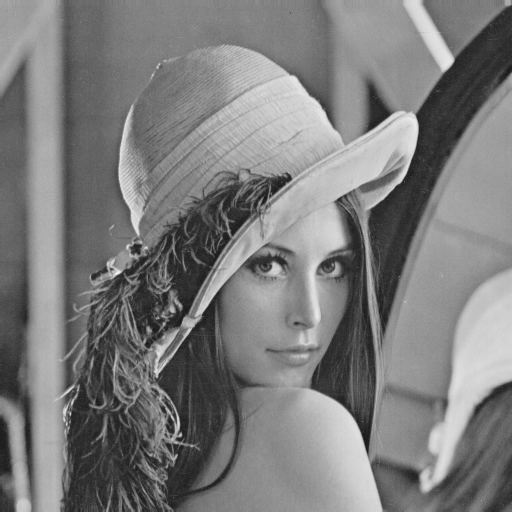
\includegraphics{/Users/dustinmayfield/Desktop/ECE418/ece418_finalproject/image/lena.png}
\caption{lena.png.}
\end{figure}

\begin{figure}
\centering
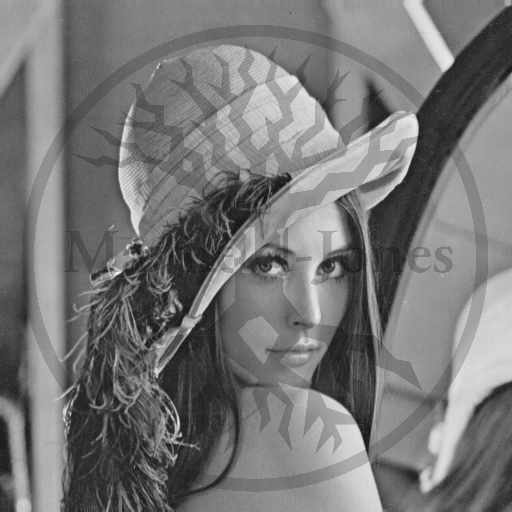
\includegraphics{/Users/dustinmayfield/Desktop/ECE418/ece418_finalproject/image/lena_basicwatermark.png}
\caption{lena\_basicwatermark.png.}
\end{figure}

\newpage

\begin{figure}
\centering
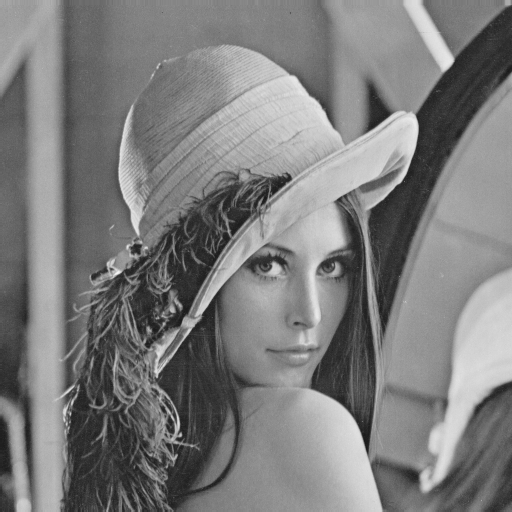
\includegraphics{/Users/dustinmayfield/Desktop/ECE418/ece418_finalproject/image/output_LSB_1.png}
\caption{output\_LSB\_1.png.}
\end{figure}

\begin{figure}
\centering
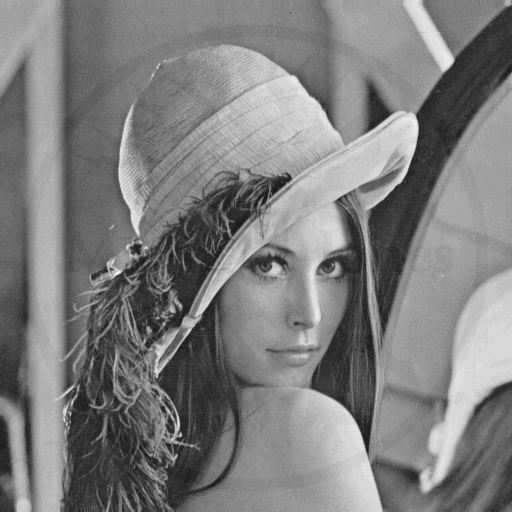
\includegraphics{/Users/dustinmayfield/Desktop/ECE418/ece418_finalproject/image/output_LSB_3.png}
\caption{output\_LSB\_3.png.}
\end{figure}


\end{document}
